%%% Demographic Research Pandoc Style
%%% Jonas Schöley
%%% 2020-08-11
%%% Depends on file "demogre.bst" for custom bibliography styling.

\documentclass[10pt, twoside, parskip=half]{article}
\raggedbottom

%%%% font/encoding %%%%%%%%%%%%%%%%%%%%%%%%%%%%%%%%%%%%%%%%%%%%%%%%%%%%%%%%%%%%

\usepackage[utf8]{inputenc}          % .tex-file text encoding
\usepackage[T1]{fontenc}             % vector fonts and special chars in output
\usepackage{times}                   % Times Roman font family

%%%% maths %%%%%%%%%%%%%%%%%%%%%%%%%%%%%%%%%%%%%%%%%%%%%%%%%%%%%%%%%%%%%%%%%%%%

\usepackage{mathrsfs} % maths script fonts
\usepackage{amssymb}  % maths symbols
\usepackage{amsmath}  % various maths features

%%%% figures %%%%%%%%%%%%%%%%%%%%%%%%%%%%%%%%%%%%%%%%%%%%%%%%%%%%%%%%%%%%%%%%%%

  \usepackage{graphicx} % include external images
  % -- We will generate all images so they have a width \maxwidth. This means
  % -- that they will get their normal width if they fit onto the page, but
  % -- are scaled down if they would overflow the margins.
  \makeatletter
  \def\maxwidth{\ifdim\Gin@nat@width>\linewidth\linewidth
  \else\Gin@nat@width\fi}
  \makeatother
  \let\Oldincludegraphics\includegraphics
  \renewcommand{\includegraphics}[1]{\Oldincludegraphics[width=\maxwidth]{#1}}

%%%% captions %%%%%%%%%%%%%%%%%%%%%%%%%%%%%%%%%%%%%%%%%%%%%%%%%%%%%%%%%%%%%%%%%

\usepackage{float}      % captions above
\usepackage[hang]{caption}
\DeclareCaptionLabelSeparator{capsep}{:\hspace{1cm}}
\captionsetup[figure]{
            labelsep        = capsep,
            name            = Figure,
            font            = bf,
            labelfont       = bf,
            justification   = raggedright,
            singlelinecheck = false
}

\captionsetup[table]{
            labelsep        = capsep,
            name            = Table,
            font            = bf,
            labelfont       = bf,
            justification   = raggedright,
            singlelinecheck = false
}

% captions above
\floatstyle{plaintop}
\restylefloat{table}
\restylefloat{figure}

%%%% localization %%%%%%%%%%%%%%%%%%%%%%%%%%%%%%%%%%%%%%%%%%%%%%%%%%%%%%%%%%%%%

% babel
\usepackage[english]{babel}         % document language/localization
\usepackage[htt]{hyphenat}          % hyphenation rules

%%%% bibliography %%%%%%%%%%%%%%%%%%%%%%%%%%%%%%%%%%%%%%%%%%%%%%%%%%%%%%%%%%%%%

\usepackage{natbib}
\setcitestyle{aysep={}}
\bibliographystyle{demogre}
\newcommand{\doi}[1]{\href{http://www.dx.doi.org/#1}{\textcolor{blue}{doi:#1}}}

%%%% layout %%%%%%%%%%%%%%%%%%%%%%%%%%%%%%%%%%%%%%%%%%%%%%%%%%%%%%%%%%%%%%%%%%%

\usepackage{geometry}
\geometry{
  paperheight = 22cm,
  paperwidth  = 17cm,
  top         = 2.54cm,
  bottom      = 2.54cm,
  inner       = 2cm,
  outer       = 2.54cm,
  footskip    = 11mm,
  headheight  = 1cm,
  headsep     = 0.75cm,
  showframe   = false
}

% change spacing
\setlength{\parskip}{0ex}
\setlength{\parindent}{.7cm}
\setlength{\bibsep}{.18cm}

% no page numbers
\pagenumbering{gobble}

% avoid orphans and widows
\widowpenalty = 10000
\clubpenalty  = 10000

% don't break footnotes
\interfootnotelinepenalty = 10000

% don't hyphenate across pages
\brokenpenalty10000\relax

% tight lists
\providecommand{\tightlist}{%
  \setlength{\itemsep}{0pt}\setlength{\parskip}{0pt}}

%%%% sections %%%%%%%%%%%%%%%%%%%%%%%%%%%%%%%%%%%%%%%%%%%%%%%%%%%%%%%%%%%%%%%%%

% spacing
\makeatletter
\renewcommand\section{\@startsection {section}{1}{\z@}%
                                   {-24pt}%
                                   {2.3ex \@plus.2ex}%
                                   {\normalfont\large\bfseries}}
\renewcommand\subsection{\@startsection{subsection}{2}{\z@}%
                                     {-24pt}%
                                     {1.5ex \@plus .2ex}%
                                     {\normalfont\normalsize\bfseries}}
\makeatother

% style
\usepackage{titlesec}
\titleformat{\section}[hang]{\raggedright\normalfont\bfseries\large}{\arabic{section}.}{1ex}{}
\titleformat{\subsection}[hang]{\raggedright\normalfont\bfseries}{\arabic{section}.\arabic{subsection}}{1ex}{}
\titleformat{\subsubsection}[hang]{\raggedright\normalfont\bfseries}{\arabic{section}.\arabic{subsection}.\arabic{subsubsection}}{1ex}{}

%%%%% footnotes %%%%%%%%%%%%%%%%%%%%%%%%%%%%%%%%%%%%%%%%%%%%%%%%%%%%%%%%%%%%%%%

% Footnotes
\usepackage[bottom]{footmisc}
\setlength{\footnotemargin}{0.6em}

% if you have code in your footnotes, the million macro march
% kind of bumps into itself.
% Pandoc, having just rendered your text into LaTeX,
% knows whether the 'variable' `verbatim-in-note` is True, and
% If it is, it asks for a  LaTeX package that solves the dilemma:

%%%% tables %%%%%%%%%%%%%%%%%%%%%%%%%%%%%%%%%%%%%%%%%%%%%%%%%%%%%%%%%%%%%%%%%%%

  \usepackage{array,longtable,booktabs,multirow}
  % -- This is needed because raggedright in table elements redefines \\:
  \newcommand{\PreserveBackslash}[1]{\let\temp=\\#1\let\\=\temp}
  \let\PBS=\PreserveBackslash
  \usepackage{etoolbox} % global table format
  \AtBeginEnvironment{tabular}{\scriptsize\sffamily}
  \AtBeginEnvironment{longtable}{\scriptsize\sffamily}

%%%% subscripts %%%%%%%%%%%%%%%%%%%%%%%%%%%%%%%%%%%%%%%%%%%%%%%%%%%%%%%%%%%%%%%


%%%% links %%%%%%%%%%%%%%%%%%%%%%%%%%%%%%%%%%%%%%%%%%%%%%%%%%%%%%%%%%%%%%%%%%%%

\usepackage{hyperref}
\hypersetup{
  hidelinks,
  breaklinks=true,
  pdftitle={An approximation to the Demographic Research style}
}

%%%% misc %%%%%%%%%%%%%%%%%%%%%%%%%%%%%%%%%%%%%%%%%%%%%%%%%%%%%%%%%%%%%%%%%%%%%

% for colored links
\usepackage{xcolor}

% Footnotes:

%%%% includes %%%%%%%%%%%%%%%%%%%%%%%%%%%%%%%%%%%%%%%%%%%%%%%%%%%%%%%%%%%%%%%%%

% header_includes

%%%% title, authors %%%%%%%%%%%%%%%%%%%%%%%%%%%%%%%%%%%%%%%%%%%%%%%%%%%%%%%%%%%

  \title{\large\textbf{An approximation to the Demographic Research style}\vskip 0em}
  \author{\normalsize\textrm{\textbf{Author 1\footnote{Here}}}\\\normalsize\textrm{\textbf{Author 2\footnote{There}}}}
\date{\vspace{-5ex}}

%%%% document %%%%%%%%%%%%%%%%%%%%%%%%%%%%%%%%%%%%%%%%%%%%%%%%%%%%%%%%%%%%%%%%%

\begin{document}

  \maketitle

\vspace*{-24pt}
\vspace*{5mm}
\setlength{\parskip}{0.5em}
\section*{Abstract}
  \noindent\textbf{BACKGROUND}\\
  What is the motivation for this submission? Why read it?
  \par
  \noindent\textbf{OBJECTIVE}\\
  What specific question(s) does this submission address?
  \par
  \noindent\textbf{METHODS}\\
  How does the submission reach its objective? What data? What methods?
  \par
  \noindent\textbf{RESULTS}\\
  What are the main findings?
  \par
  \noindent\textbf{CONCLUSIONS}\\
  What do the findings mean?
  \par
  \noindent\textbf{CONTRIBUTION}\\
  What new contribution does this submission make to the scientific
  literature?
\vspace*{12pt}

\setlength{\parskip}{0ex}

\hypertarget{figures}{%
\section{Figures}\label{figures}}

When it comes to proportions, the number ``three'' is quite significant:
the share of people working in the primary vs.~secondary vs.~tertiary
sector, the proportion of total population change explained by migration
vs.~fertility vs.~mortality, the relative population numbers in young
age vs.~working age vs.~retirement age, the share of a cohort attaining
primary vs.~secondary vs.~tertiary education degrees, the relative
number of deaths due to prematurity vs.~accidents vs.~old age, the share
of papers accepted as is vs.~revised vs.~rejected\ldots{} three-part
proportions of a whole, i.e., ternary compositions, are a type of data
that is both ubiquitous and idiosyncratic enough as to warrant
particular attention when it comes to presentation. The ternary diagram
and its use throughout the sciences stand as a manifestation of this
view.

Variably referred to as de Finetti-, simplex-, or triangle plot, the
ternary diagram is based upon a coordinate system that maps each point
within an equilateral triangle to a unique three-part composition and as
such has found use wherever the problem domain spans three parts of a
whole. The diagram emerged during the 18th century as a means of
illustrating relative mixtures of primary colors \citep{Howarth1996}. It
was subsequently adopted as the standard method to depict phase
transitions in three-component alloys \citep{Bancroft1897}, the genotype
composition of a population \citep{DeFinetti1926}, soil composition
\citep{Davis1927}, or the potential for flammability given different
mixtures of three gases \citep{Zabetakis1965}. In the social sciences,
ternary diagrams depict population compositions along demographic
characteristics, with an early example appearing in the USSR's first
census report showing the distribution of workers across labor market
segments in various regions \citep{Kvitkin1932}.

\begin{figure}
\centering
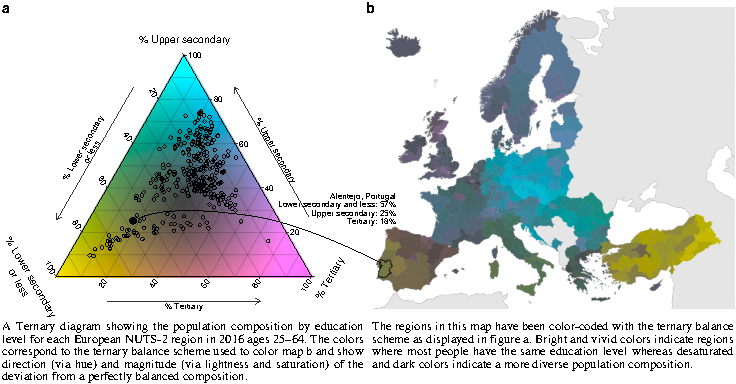
\includegraphics{figure1.pdf}
\caption{Demonstration of the ternary balance scheme showing the
composition of educational attainment by region in Europe 2016. Data by
Eurostat.}
\end{figure}

Wherever three-part compositions are available by geographical region or
other pairs of ordered attributes such as cohort and age, one faces the
challenge of visualizing ternary compositions on a surface such as the
surface of the Earth or the period-age Lexis surface. The \emph{ternary
balance scheme} \citep{Brewer1994} is a color scale suited to that task.
The technique encodes the relative shares among three parts as a mixture
of three primary colors. Figure 1B shows the proportions of people with
either ``lower secondary or less,'' ``secondary,'' or ``tertiary''
educational attainment by European region in 2016. Lower degrees are
mapped to yellow, secondary to cyan, and tertiary to magenta. The more
pronounced the yellow in a region, the higher the share of people with
lower education. The same logic applies to the two other education
categories. The more grayish a region is colored, the more balanced the
three proportions are with a perfect grey signifying an equal share of
people in all three education categories. A ternary diagram is used as a
color key (see Figure 1A) and doubles as a visualization of the
distribution of data marginalized over the geographical surface.

Published examples of the ternary balance scheme include maps of
population compositions by political alignment, education and workforce
status \citep{Dorling2012, Graetz2019, Brewer1994}, geological maps of
soil composition \citep{Metternicht2003}, arctic sea ice coverage by
type \citep{Denil2015} or land cover compositions by type of forest
\citep{Pirzamanbein2020, Steidinger2019}. \citet{Schoeley2017} employed
the scheme to visualize the distribution of deaths by cause among the
French population on a period by age surface.

\begin{figure}
\centering
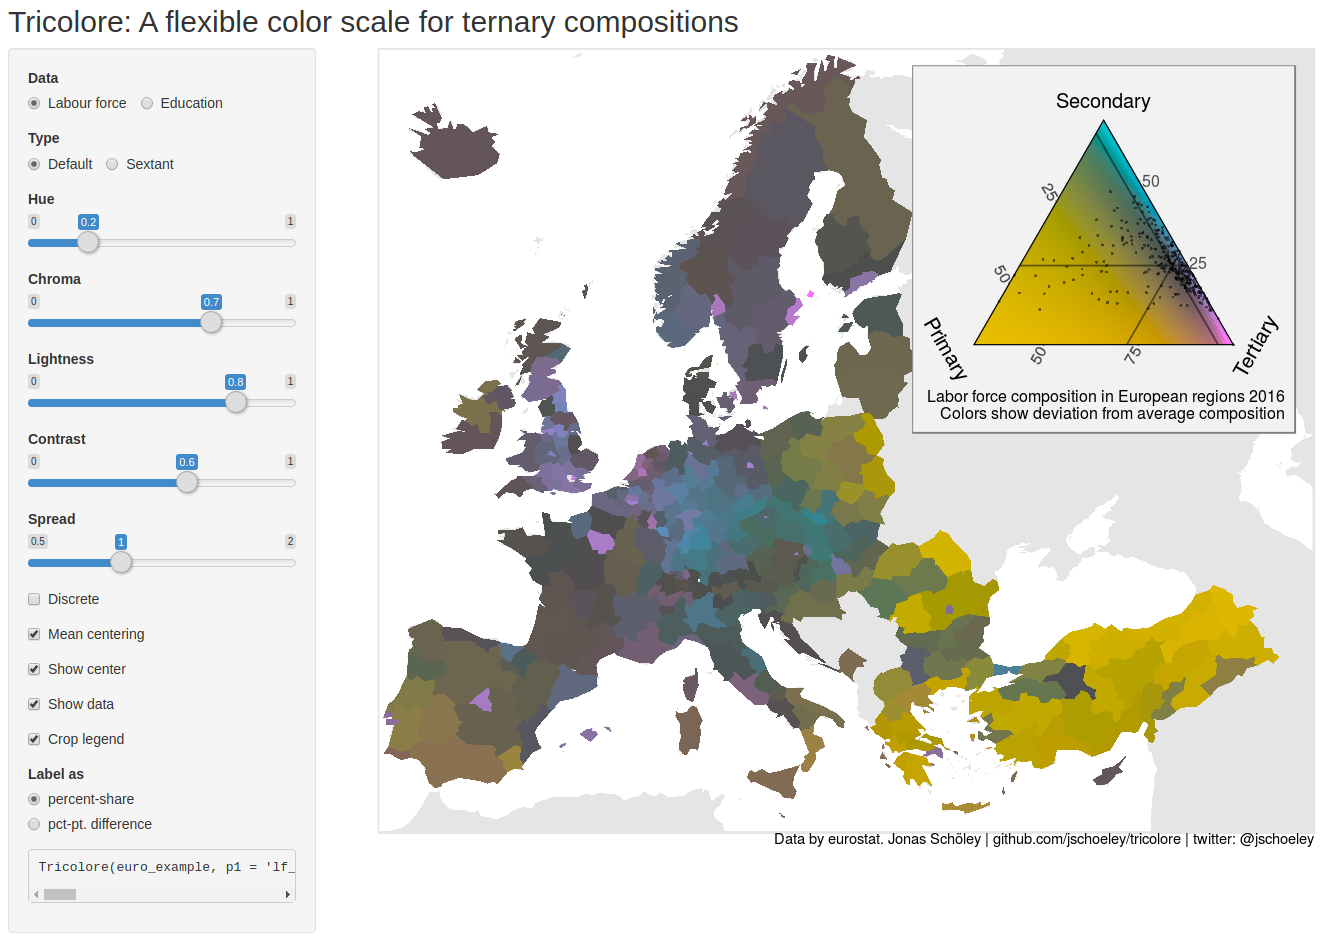
\includegraphics{figure2.png}
\caption{The ``tricolore'' package for the statistical programming
language R implements the centered ternary balance color scheme and
provides a user interface for quickly testing different
parametrizations.}
\end{figure}

\hypertarget{tables}{%
\section{Tables}\label{tables}}

\begin{longtable}[]{@{}rrrrl@{}}
\caption{A table.}\tabularnewline
\toprule
Sepal.Length & Sepal.Width & Petal.Length & Petal.Width &
Species\tabularnewline
\midrule
\endfirsthead
\toprule
Sepal.Length & Sepal.Width & Petal.Length & Petal.Width &
Species\tabularnewline
\midrule
\endhead
5.1 & 3.5 & 1.4 & 0.2 & setosa\tabularnewline
4.9 & 3.0 & 1.4 & 0.2 & setosa\tabularnewline
4.7 & 3.2 & 1.3 & 0.2 & setosa\tabularnewline
4.6 & 3.1 & 1.5 & 0.2 & setosa\tabularnewline
5.0 & 3.6 & 1.4 & 0.2 & setosa\tabularnewline
5.4 & 3.9 & 1.7 & 0.4 & setosa\tabularnewline
\bottomrule
\end{longtable}

\newpage

\bibliography{references.bib}

\end{document}
